\documentclass[10pt,a4paper]{article}

\usepackage[english]{babel}
\usepackage[utf8]{inputenc}
\usepackage{amsmath}
\usepackage{graphicx}
\usepackage{todonotes}
\usepackage{url}

\title{Extensions on Contract Net Protocol for AGVs \\ \normalsize Multi-agent systems}

\author{Jens Claes \and Victor Le Pochat}

\date{June 3, 2016}

\newcommand{\proposalY}[1]{\todo[inline, color=green]{Proposal (by Yens): #1}}
\newcommand{\proposalV}[1]{\todo[inline, color=green]{Proposal (by Victor): #1}}

\newcommand{\commentY}[1]{\todo[inline, color=yellow]{Yens: #1}}
\newcommand{\commentV}[1]{\todo[inline, color=yellow]{Victor: #1}}

\newcommand{\taskY}[1]{\todo[inline, color=red]{@Yens, fix: #1}}
\newcommand{\taskV}[1]{\todo[inline, color=red]{@Victor, fix: #1}}
\newcommand{\taskS}[1]{\todo[inline, color=red]{@???, fix: #1}}

\newcommand{\outline}[1]{\todo[inline, caption={}, color=cyan]{\emph{Outline of what should come here}: #1}}

\graphicspath{ {./vpp/} }

\begin{document}
\maketitle

\commentY{In 2 kolommen? => geeft wel ander aantal pagina's, dus opletten met theorie sectie dan. Maar in mijn ogen is het wel een pak beter\commentV{In finaal verslag: ja - veel beter; in werkdocument zou ik het afzetten zodat we een goed idee hebben van de lengte}}

\section{Introduction}
\proposalY{Nog voor Objectives een context sectie hebben?}
\commentV{Zie https://bitbucket.org/VictorLP/mas/wiki/Notities}
\commentY{Normaal staan alle comments van de wiki in het verslag nu}
\commentV{The last paragraph of the introduction traditionally says “This report is organised as
follows. Section 1 introduces . . . ”.}
\subsection{Objectives}
\outline{\proposalV{Investigate the performance changes between DynCNET/confirmation and CNET. (bijbehorende question: what is the relative performance of cnet, confirmation and dyncnet)}}
The objective of this paper is to compare 2 extensions of Contract Net (CNET)\cite{CNETStandard,CNET}, namely Contract Net with Confirmation Protocol (CNCP)\cite{CNCP} and Dynamic Contract Net (DynCNET)\cite{DynCNET} to CNET itself. \commentV{extensions should be measurable \proposalV{to investigate whether these two extensions (CNCP/DynCNET) are an improvement on CNET\commentY{akkoord}} }

We do this in a drone delivery setting where all agents (both the drones and the clients) try to maximize (locally) the profit for the company. Drones can fail and are constrained by their batteries. The company needs to pay a fine for every client that is not delivered in time. The drones can pick up the packages in multiple warehouses (with infinite stock), each with a different price per package. Drones cannot collide with each other.
\commentY{De setting moet nog serieus herschreven worden, bovenstaand stukje is niet duidelijk. Zeker in vergelijking met sectie 2: Context van de opgave.\proposalV{We do this in a drone delivery setting where a company owns a fleet of drones that receives orders from clients, collects the ordered parcel at one of several warehouses and delivers them to that client. The drones autonomously receive, process and deliver the client orders. The goal is to maximize the company's profit, by having the most suitable drone serve each order. Clients have a time limit for their deliveries, after which the company needs to pay a fine.  Drones can break down and are constrained by their batteries. Drones cannot collide with each other.\commentY{Al een pak beter. nog paar kleine dingen: - parcel of package: moeten 1 term gebruiken voor heel het document, denk ik. - Niets over waar opladen?}}}

We investigate whether any of the aforementioned protocols are suited for a drone company to be profitable in the described setting. We will also check the influence of the number of drones, clients and warehouses on the profit the company can make.
\subsection{Hypotheses}
We formulate the following questions and provide our hypotheses for the answers to them.
\begin{itemize}
\item \textit{Is there a difference between CNET, CNCP and DynCNET in the profit the company can make?} \\
We expect that the company can make more profit using DynCNET than using CNCP, which should be more profitable than CNET.
\item\textit{Is there a difference in average delivery time between CNET, CNCP and DynCNET?} \\
We expect that CNCP and CNET will deliver faster than DynCNET (as DynCNET wastes time when it switches). We don't expect a difference between CNCP and CNET as both will start delivering fast and won't waste any time by switching.

\item\textit{Is there a difference in the number of clients that are not delivered between CNET, CNCP and DynCNET?} \\
We expect that CNET and CNCP will deliver the same amount of clients and DynCNET less. Again because of the switching between clients.

\item\textit{Is there a difference in the number of messages that needs to be exchanged between CNET, CNCP and DynCNET?}\\
We expect that CNCP will need less messages because we expect less rounds of bidding. CNET will take more messages but still less than DynCNET which needs a lot of messages to make sure the best contract is being executed. 

\item\textit{Is it possible to make a profit using any of the 3 approaches?}\\
We expect that all 3 approaches should be profitable give the right number of warehouses, drones and clients.

\item\textit{What is the influence of the number of drones on the profit?}\\
We expect the profit to scale linearly with the number of drones. Once all clients start to get delivered, saturation will set in.

\item\textit{What is the influence of the number of warehouses on the profit?}\\
We expect the profit to scale with the number of warehouses. As more warehouses become available, it will become more likely to have a warehouse with a low price for the product near the customer.

\item\textit{What is the influence of the number of clients on the profit?}\\
We expect the profit to rise until the fines of not delivering start to become too large.
\end{itemize}

\outline{In profit: DynCNET better than Confirmation better than CNET \\ In messages: CNET better than confirmation better than DynCNET\commentY{Done?}}

\section{Theory}
\outline{Theoretische uiteenzetting van wat in de drie relevante papers staat}
\commentV{Theory nog iets algemener, meer van onze eigen dingen in system design zetten? zie ook hoofdstuk 7 Schut\commentY{jup}}

In this section we describe the theory of the Contract Net Protocol and the two extensions CNCP and DynCNET. We use the literature on these protocols to highlight their characteristics and differences.

\proposalY{In this section we describe how the theory of multi-agent systems maps onto our implementation. We first discuss the theory of contract net, followed by the variations made in CNCP and DynCNET. We conclude with a description of the agent architectures.}

\taskS{Add sequence diagrams of 3 protocols (mss met kleuren werken om verschillen aan te duiden?). Best met zelfde kleuren als grafieken dan: CNET rood, CNCP groen en DynCNET blauw\commentY{Als we het doen, dus in design sectie?}}

\subsection{Contract Net} The Contract Net Protocol, or CNET, was conceived by Smith in 1980. \cite{CNET} It is a high-level protocol for communication between agents to allow distributed task execution. The high-level protocol messages have a particular structure and meaning, which means the agents can interpret them to receive information on tasks and allocations and to send replies such as bids. 

CNET tries to solve the problem of assigning tasks to idle agents in the most efficient way. Moreover, this problem needs to be solved in a distributed manner, without a central authority that tracks tasks and assigns them with global knowledge.

CNET relies on the negotiation of contracts between a manager and a contractor for the execution of a task. The manager (or initiator) launches a tender for the execution of a task and will monitor the execution and process the results once they arrive. The contractor (or participant) bids on the tenders and when it wins, executes the task and submits the results to the manager. Each agent can be one of these roles for each individual task. This can also mean that an agent acts as a contractor for one task and as a manager for sub-tasks of this task to distribute the workload over several agents.

The Contract Net Protocol is defined by the messages and the information that is contained within them. By having a common language for these messages, all agents can communicate with each other and new agents can immediately start listening for new messages and participate in the negotiation process. There are three types of messages: those related to task announcements, those related to bids and those for the reporting of task results.

A manager initiates the contract negotiation process by adversiting that task with a task announcement message. This message can either be broadcasted to all agents or sent only to one or a few nodes in a focused manner. The task announcement message contains four main parts: an eligibility specification, a task abstraction, a bid specification and an expiration time. The eligibility specification describes what criteria an agent must meet to be able to bid and eventually possibly receive the contract and execute the task. The task abstraction is a description of the task to be executed. The bid specification outlines the expected form of a bid. The expiration time marks the final time at which a bid may be submitted.

Whenever a task announcement arrives at an agent that wants to act as a contractor, all of these parts of the announcement allow contractors to decide whether and when to submit a bid. They add the announcement to a list of received and not expired announcements if they're eligible. The announcements in the list are ranked on interest to the agent. This ranking is a task-specific operation and is based on the information contained within the task announcement.

A busy agent cannot bid while busy, but continues to process the task announcements while executing its task. When this task completes, it can then check the list of task announcements and pick a task to submit a bid on. An idle agent will decide to bid on a task either immediately when it arrives or when it expires. It either submits a bid to the most interesting task or waits for new (better) task anouncements. In a bid, an agent describes its specification in the node abstraction slot. It can also indicate additional information that will be required if the agent may execute the task. Whenever an agent submits a bid to a task, it is bound to that task. This is also called early commitment. This means that it cannot bid on other tasks and already allocates its resources to that task. Only when the task expires and no message is received that the contract has been awarded, can the agent release its resources and bid on other tasks. This is done to avoid multiple task awards to one agent, which would need to be queued and would slow down the system performance. It does mean idle agents are 'blocked' until their bid is rejected, but this is reduced by allowing bids and awards before the expiration time. \commentV{klopt dit? staat precies wel in de paper maar klinkt zo raar (vooral: agents die niet awarded worden moeten toch wel nog tot expiration wachten -- zie ook FIPA) \commentY{Nee, Contract Net laat dit wel toe. Alleen moogt ge niet op 1 tijdstip 2 bids uitsturen. Ge moogt wel een tijdstip later bieden als ge dan nog altijd geen contract hebt. Zie sectie IV.A.6:Negotiation Tradeoffs dat gaat hierover}}

Bids arrive at the manager and are also ranked and stored in a list until the task can be awarded. The manager can either award a contract immediately if a satisfactory bid arrives (even before the expiration time) or wait for further bids. When the task expires\commentY{Task expiret niet, de task announcement eerder}, it can either award the contract to the best bidder in its list or advertise the task again \proposalY{later on}. The task is therefore not necessarily awarded when it expires. If a manager awards a contract, it sends a message to the winning contractor, who can start executing the task. When the contractor is finished, it sends a report to the manager with the results of the execution.

The bidding process can be extended to allow agents that cannot or do not want to bid to respond immediately with their reason why they will not bid. Managers can then delay task announcements if no agent is ready to take up the task. An agent can respond immediately if they are ineligible, busy or give the task a low ranking. The manager can then avoid simply reissuing the task announcement when it expires, but can loosen the eligibility requirements if all agents are ineligible or wait before reissuing the task announcement if all agents are busy or not interested yet in the task.

The FIPA version of the Contract Net Protocol \cite{CNETStandard} differs from the original protocol by adding acceptance and rejection of a bid by a manager. This means a contractor is notified if its bid was rejected, which means it does not have to wait until the task expires to continue bidding on other tasks.
\commentY{laatste bijzin weg, komt nog uit foute interpretatie van CNET}

\subsection{Contract Net with Confirmation} 
The Contract Net With Confirmation Protocol, or CNCP, was conceived as an extension to the Contract Net Protocol by Knabe et al. in 2002. \cite{CNCP}

The major shortcoming of CNET that CNCP tries to address is the early commitment by agents. If multiple managers announce a task, a contractor is only allowed to bid on one of the tasks and must then allocate its resources to that task and cannot bid on other tasks, even though it might not be awarded the task. 
\commentY{Deels terug die foute interpretatie CNET. Early commitment is wel juist. Biedingen op andere tasks moeten rekening houden met het feit dat er minder resources zijn want een deel is al toegekend aan bids die uitstaan (en die soms pas tegen expiration time een antwoord krijgen)}

To resolve this issue, in the CNCP the full commitment to a task is moved to the awarding phase: if a contractor is awarded a task, only then does it allocate its resources and stop bidding on other tasks. While a bid has been submitted but the task has not been awarded yet, the contractor can continue bidding on other tasks. When a manager wants to award a task to a contractor, it first contacts that contractor with the request to accept the task. This contractor may however already been awarded a different task, in which case it will refuse the task. The manager may then try to award the task the next best contractor. This either continues until a contractor accepts the task, in which case the contractor can start executing the task and the manager can send a rejection message to the other bidders, or if no contractor accepts it, the manager can announce the task again (possibly after waiting some time).

CNCP requires two more messages to allocate a task: one to request the execution of a task by the manager and one reply to this message by the contractor. If the first contacter bidder refuses, the next best bidder has to be tried and two messages need to be sent. In the worst case this means 2$n$ extra messages (with $n$ the number of bidders) must be sent.

\subsection{Dynamic Contract Net}
The Dynamic Contract Net Protocol, or DynCNET, was conceived as an extension to the Contract Net Protocol by Weyns et al in 2007. \cite{DynCNET}

DynCNET tries to improve on CNET by adding dynamism to the allocation and execution of tasks. More specifically, it addresses the fact that an agent usually has to do some preparation when it is assigned a task before it can actually start executing this task. DynCNET allows contracts to be switched during this preparation phase.

DynCNET changes the acceptance of task by a winning contractor to a provisional acceptance. This means that until further notice that contractor will execute the task and report the results. The contractor can then start its preparation for the execution of the task. During this preparation phase however, the contractor is free to continue bidding on other (new) tasks and the manager may continue announcing the task. If either receives an offer that they consider better than the current contract, they are allowed to cancel the current contract and pursue another task. As soon as a contractor finishes its preparation and starts the actual execution of the task, the contract is final. The contractor is fully committed to the task and no longer bids on other tasks. The contractor also notifies the manager that it is executing the task, which means the manager stops announcing the task.

The synchronization between managers and contractor to assess their current state requires some additional messaging. If a manager cancels a contract, it needs to notify the original contractor that the task has been awarded to another agent. Inversely, a contractor that takes up another task needs to notify the manager of the original task that it is no longer committed to executing that original task. Finally the contractor needs to send a message to the manager when it starts executing the task, so the manager can stop announcing the task to other agents.


\subsection{Agent Architecture} 
\commentV{waar moet dit best komen?\proposalY{Ik zou het er nu misschien zelfs uitlaten. Daarvoor was het ook deels nodig om aan onze 3 pagina's te komen. Dus bij design eventueel wel nog FSM's zetten, maar zeker niet "Agent Architecture" erbij zetten.}}
Both the drone and client agents have very simple architectures. They can be modeled using simple finite state machines.

Figure~\ref{fig:droneFSM} gives the FSM for the drone agent in the different protocols\footnote{Not represented in the figure is the failed state, in case the drone crashes. A drone can enter this state from all other states and can never leave it again}. The \texttt{PROPOSED\_BID} state is only used in CNET, not in CNCP nor DynCNET. In CNET and CNCP, a drone can bid in the green states. In DynCNET, a drone can bid in the green and yellow states. DynCNET also has two extra transitions: from \texttt{PICKING\_UP} and \texttt{CHARGING\_FOR\_CONTRACT} back to \texttt{IDLE} in case the client cancels the contract. CNCP and DynCNET also have the \texttt{gotContract} transition from \texttt{IDLE} and \texttt{CHARGING\_FOR\_CONTRACT} to \texttt{PICKING\_UP}, while in CNET the drone has to pass through the \texttt{PROPOSED\_BID} state.

\begin{figure}[htp]
    \centering
    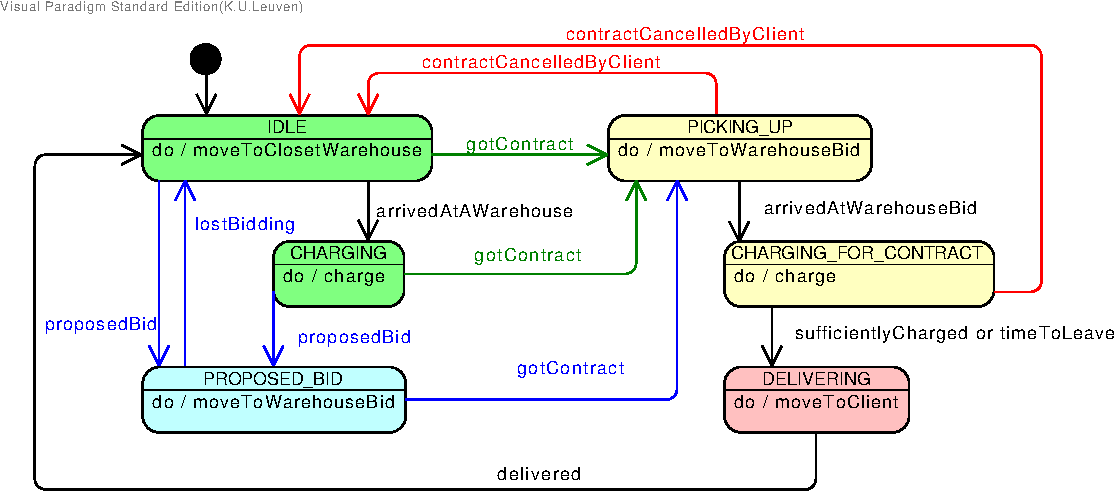
\includegraphics[width=\columnwidth]{Drone}
    \caption{A finite state machine of the drone agent (the blue transitions and state only apply to CNET. The red transitions only to DynCNET and the green transitions to CNCP and DynCNET)}
    \label{fig:droneFSM}
\end{figure}

\commentY{Ook "biedingen" beter op FSM weergeven? Of dat laten voor sequence diagram}

The drone starts of in the \texttt{IDLE} state. In this state, it will move to the closet warehouse. When it gets there, it will enter the \texttt{CHARGING} state and start charging. In CNET, a drone will enter the \texttt{PROPOSED\_BID} state once it has sent a bid to a client. It will reenter the \texttt{IDLE} state if the client declines or move to the \texttt{PICKING\_UP} state when the client accepts. In the \texttt{PICKING\_UP} state it will start moving to the cheapest warehouse. When it gets there, it will start charging until it is sufficiently charged or it is time to leave (because the deadline of the client is coming up). Then it will pick up the package and enter the \texttt{DELIVERING} state. From then on, it will keep flying to the client until it has arrived, upon which it will deliver the package to the client and enter the \texttt{IDLE} state.

\begin{figure}[htp]
    \centering
    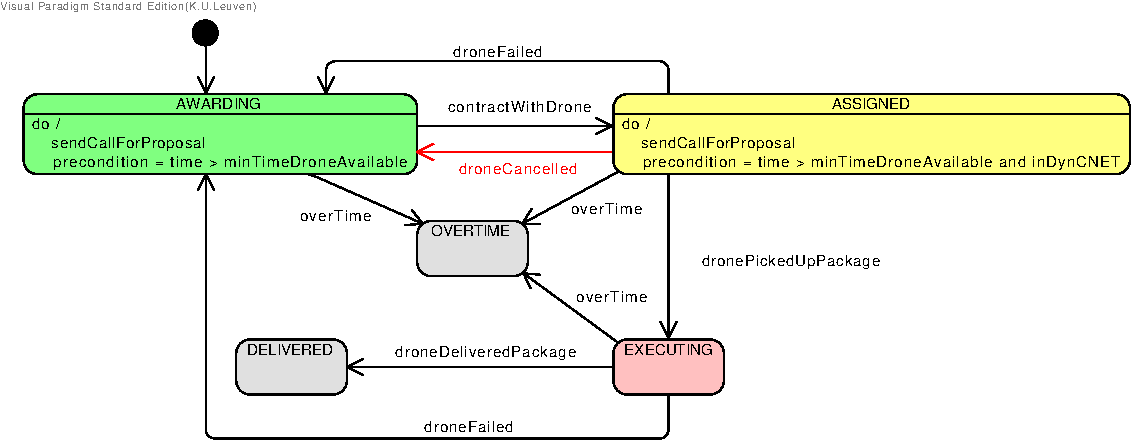
\includegraphics[width=\columnwidth]{Client}
    \caption{A finite state machine of the client agent (the red transition only applies to DynCNET)}
    \label{fig:clientFSM}
\end{figure}

The client FSM, in figure~\ref{fig:clientFSM}, is even simpler. The clients starts in the \texttt{AWARDING} state. When a contract is negotiated, it enters the \texttt{ASSIGNED} state. From then on, it is a straight path to the \texttt{EXECUTING} and \texttt{DELIVERED} state. Only a drone failure, or the cancellation of a contract in DynCNET, can change the state flow. If the maximum delivery time for the client has passed before a drone delivered the package, the client will enter the \texttt{OVERTIME} state.

In CNET and CNCP, a client can only send calls for proposals while in the \texttt{AWARDING} state. In DynCNET, it can also send calls for proposals in the \texttt{ASSIGNED} state.

\commentY{Table met communication primitives as in \cite{TentativeBidding}?}


\section{Multi-agent system design}
\outline{Wat wij concreet doen}
\subsection{Design}
\outline{\begin{itemize}
        \item drones leveren orders uit warehouses aan clients (1 order per client)
        \item bid berekening (statistisch relevant)
        \item messaging gedetailleerd bespreken of niet?
        \item tijd tijdens opladen wordt niet meegerekend bij estimated cost (footnote)
    \end{itemize}}
    
\proposalY{\textbf{CNET: } Our system has two types of agents: clients (who represent a package that needs to be delivered) and a drone. The two types of agents each fulfill a different role in CNET: clients fulfill the role of manager, while the drones fulfill the role of contractor. When clients enter the world, they will announce a call for proposal to all agents \textbf{footnote}{This includes other clients, which will ignore all calls for proposals. RinSim does not (yet) provide a broadcast to a subset, the drones, of all agents.} through the means of broadcasting. This task announcement is simplified from the original paper \cite{CNET}. As all drones are eligible, no eligibility information is provided. The bid specification is missing as well. There is no expiration time on the call for proposal, as drones should bid as quickly as they can.
    
When drones receive task announcements, they will calculate, for every warehouse, the estimated profit \textbf{footnote}{Taking the delivery window and the probability of a crash into account} they can make on this client. Only the warehouse with maximal profit for the client is kept. This is done for all task announcements. A drone is only allowed to bid on 1 of those announcements, therefore the most profitable client is selected \textbf{footnote}{If it is economically better to not deliver any client, no bids are placed}. A propose message is sent to this client including the estimated profit the company can make on this client. Once a drone has placed a bid, he will enter the \texttt{PROPOSED\_BID} state in which he is no longer allowed to bid until either he is awarded the task and has executed it or the client refuses his bid.

When a client receives a bid, it will compare it to the other bids it got (if any) and will award the contract to the drone which will make the most profit for the company  \textbf{footnote}{The client agent thus acts as if it is the manager, responsible for the real client, trying to maximize the profit the company can make on this client}. It will send the drone a message to inform him of the contract. All other drones will be informed that their proposal has been declined. If later on, more proposals would arrive, the client will decline them as well. 

Because drones won't bid if it is not economically interesting, all bids are satisfactory for the client.

Once the drone has received the contract from the client, it will start executing it. After picking up the package at the warehouse, the drone will inform the client about this. When it has delivered the package, a message is sent as well. In case the drone would crash, it would sent one last signal to the client to inform him of the crash \textbf{footnote}{In practice, outside a simulator, a polling approach might be used instead.}. The client would then start sending out calls for proposals again.

As said earlier, once a bid has been placed, a drone cannot bid unless the current task has been executed or his bid was declined. While \cite{CNET} suggest that this might increase delay significantly, we assumed the effect would be smaller in our design where clients assign contracts from the moments they receive bids. As a drone can only hold 1 contract, there is no need for a local scheduler within the drone.

To reduce the message count significantly, drones send explicit refuse messages to clients (as answer to a call for proposal). In these messages, the reason for refusal is added. There are 3 possibilities: \texttt{BUSY} \textbf{footnote}{The drone is executing another delivery}, \texttt{LOW\_RANKING} \textbf{footnote}{The drone prefers the proposal of another client.} and \texttt{INELIGIBLE} \textbf{footnote}{It is not economically profitable for the drone to deliver to this client}. Clients will act smart based on these refusal reasons. If a \texttt{LOW\_RANKING} is received, it can send a new call for proposal immediately as it is likely that a drone was refused the contract it preferred. If only \texttt{BUSY} or \texttt{INELIGIBLE} refusals are received, a new immediate call for proposal has little chance of succeeding. We know that the drones are busy delivering other packages or are too far away. Clients can thus wait until a drone becomes available again. \cite{CNET} suggests that drones could declare when they are available and what kind of tasks they can execute so the clients can propose them instead of the other way around. We decided to give extra information to the refusal message: If busy, the refusal message also contains a lower limit on when the drone will become available again. The client can now wait with sending out new calls for proposals until this lower limit has passed.}

\proposalY{\textbf{CNCP:} The earlier solution suffers from 1 major flaw: drones have to commit to their bid until the client accepts or declines their bid. They are not allowed to bid on other task announcements while they have a bid outstanding. As their are $n$ drones and $m$ clients, $n*m$ bids are possible in theory. In practice, only $n$ bids are sent out. In the worst case, where all drones rank the clients in the same order $O(m)$ rounds of bidding are necessary to assign all clients to drones in CNET.

In CNCP, the drones are allowed to sent out multiple bids. Only when a drone receives an \texttt{AcceptProposal} message, should it commit to a bid. In case it receives multiple bids, it can choose to which bid to commit. The client to which is committed is sent an \texttt{Agree} message. From that moment on, the drone starts executing the delivery \textbf{footnote}{In \cite{CNCP} they first sent a \texttt{Request} message and only upon the \texttt{Agree} message of the client, the \texttt{AcceptProposal} is sent. These two messages from the client to the drone are merged together in our design}. All other clients are sent a \texttt{Disagree} message. When a client receives a \texttt{Disagree} message, it will send out a new call for proposal. This behaviour differs from \cite{CNCP}: when a client receives proposals, it will rank them and send out an \texttt{AcceptProposal} to the first one. If the first drone declines, the second drone will be sent an \texttt{AcceptProposal} and so on, until all (satisfactory) drones are sent an \texttt{AcceptProposal}. Because of the short deadlines and the high chance that the second drone has in the mean time committed to another client, we preferred to start a new bidding round.
\commentY{Disagree: note van dat dit een ACL-refuse message is? of via diagram?} 

While CNCP as described in \cite{CNCP} requires an extra $O(2*n)$ messages, our design only requires one extra message per bidding round. We believe the number of bidding rounds will be reduced drastically, and therefore the total message count as well (compared to CNET).}

\proposalY{\textbf{DynCNET: }

CNCP still suffers from one problem: while a drone is flying to the warehouse (and while he is charging in the warehouse before delivering the package), the world might change. Maybe another drone becomes available, or another client announces a new task. In both scenarios, it might be better to cancel the contract and start a new one. Neither CNET nor CNCP allow a drone or client to change a contract after they have committed to each other. In DynCNET, a drone can still cancel the contract, as long as it has not yet picked up the package in the warehouse. So if a better client comes along, a drone could cancel the old contract and start a new contract with this new client. Similarly, a client can break up the contract with a drone as long as this drone has not yet picked up the package. If a better drone becomes available (after it has delivered another package), the client might switch drones. It will let the old drone known that the contract has been canceled.

This means that in practice, the client will keep sending calls for proposals until the drone has picked up the package. Similarly, the drone will keep bidding on task announcements until it picks up the package. From then on, both agents are 100\% committed to the contract.

A potential risk of DynCNET is oscillation of tasks between drones. \cite{DynCNET} describes a solution by limiting the areas of interest. In our design, the agents are only limited by the battery constraint of the drones. We did not take special action to prevent the oscillation of tasks between drones.


\commentY{Message loss?}

\commentY{Synchronization van DynCNET: }
\commentV{This latter then sends a message to confirm the abort.
moeten we verbreken contract bevestigen? zie DynCNET + CW566: 3.3. Synchronization of abort messages}
}
\subsection{Comparison with existing MAS from literature}
\outline{
    \begin{itemize}
        \item warehouses oneindige capaciteit
        \item tasks uit literature zijn orders bij ons
        \item verschillen in messaging
        \item concretere berekening bid
        \item hier de state machines? (of eerder bij design)
        \item Feit dat ze enkel kunnen opladen als ze IDLE (CHARGING) zijn of in CHARGING\_FOR\_WAREHOUSE? En dus niet in andere warehouses. En ook niet voor ze naar andere warehouse vertrekken.
    \end{itemize}
    }
\commentY{\cite{TentativeBidding}, \cite{LeveledCommitment}, \cite{CNETIterativeStandard}, zie ook \cite{DynCNET} Related work voor korte beschrijving}
\commentV{misschien bij theory gedeelte?\commentY{Wat bij theorie gedeelte?}}

\taskS{Nu altijd geschreven als client-drone, aanpassen naar initiator-participant, om te matchen met theorie sectie + eventueel eens kijken dat zelfde termen gebruikt worden}

In the literature, other extensions of CNET can be found. \cite{TentativeBidding} describes a 2-phase protocol (PreBidding and DefinitiveBidding). The first round of pre-bidding is only tentative. The client informs the drones of the tentative results. Drones can still change their offers based on this tentative results and how the world (and other bidding processes) evolve. Once a drone has been tentatively accepted, it can send a definitive bid to the client. If this bid is still better than all tentative bids from other drones, the drone will be informed and both agents commit to the contract. All other drones will be informed that the bidding is definitely over. If the definitive bid is not the best bid, the drone gets tentatively or definitely declined. In case of the former, it can submit a new tentative bid. This protocol can be seen as an extension on CNCP. Drones who get accepted, can accept or decline by choosing the appropriate definitive bid. The advantage of this protocol is that drones who get rejected can still improve their bid.

\cite{CNETIterativeStandard} describes a similar protocol: iterated contract net (ICN). When a client receives bids, it can choose to accept one, or choose to iterate the process by issuing an adapted the call for proposal to a subset of the bidders. The intent of this next iteration is to receive better bids. The protocol stops when a drone is awarded the contract, the client stops issuing calls for proposals (because all bids are unsatisfactory) or all drones stop bidding.

The tentative bidding of \cite{TentativeBidding} and ICN are very similar. Both protocols can be mapped onto each other.\commentY{Dat erin laten van het mappen op elkaar? Ik denk dat dat het geval is, als ik diagrammen vergelijk, maar niet 100\% zeker} One of the main differences is that ICN issues new calls for proposals and can thus actively try to increase the price of the contract.  In our setting however, both protocols do not make much sense. Drones bid using the estimated profit. They cannot increase their bid, unless the estimated profit changes.

\cite{LeveledCommitment} uses game theory to proof that leveled commitment is to be preferred in all situations over full commitment. In the negotiation of a contract, a decommitting penalty is agreed upon. (This penalty might be different for both agents). When an agent wants to cancel the contract, he has to pay his decommitting fee to the other agent. This not only gives a way to calculate whether or not to cancel a contract in favor of another contract\footnote{They prove (again using game theory) that it is harder than just checking if the profit of the new contract is higher than the fee, because the other agent might decommit if this agent doesn't decommit.}. It also allows contracts that were not possible using full commitment: it is possible that the benefit from a contract is lower than the expected benefit from other contracts that have not yet been announced. But by having the right decommitting fees, a leveled commitment contract might still be interesting for both parties.

It is important to note, that in our design, bids are satisfactory if the expected profit is above the fine for not delivering to this client. (It does not take into account that new clients or drones might become available). The agents described in \cite{LeveledCommitment} take the expected profit of new clients or busy drones into account.

\section{Experiments}
\subsection{Setup}
\outline{\begin{itemize}
        \item independent: aantal drones, warehouses, clients
        \item dependent: profit, aantal clients delivered, aantal messages, delivery time, ... (\texttt{ExperimentResult})
        \item other: battery drain, kost pakketjes, oplaadkost, ... (\texttt{Variables.kt} + \texttt{PackageType.kt})
        \item beschrijving computer + RinSim 4.1.0
    \end{itemize}}
\subsection{Results}
\commentY{Ook 95 \% Confidence interval (CI) op grafieken? Prof is daar precies fan van => Misschien beter om te doen. Ik ben niet 100\% zeker van correctheid, maar misschien wel, omdat het CI is van de variabele, niet het verschil tussen 2 variabelen. Dus zolang variabele normaal verdeeld is, is het waarschijnlijk wel ok.}
\subsection{Analysis}
\commentY{Reference Statistische modellen en data-analyse boek van Mia Hubert voor onze statischische methodologie}

\section{Conclusion}
\commentV{CW566: TABLE 1: INTERFACE DEFINITIONS FOR A TRANSPORT AGENT AND AN AGV AGENT
nakijken of we die allemaal hebben}
\commentY{Ook http://www.fipa.org/specs/fipa00037/SC00037J.html als referentie voor de ACL acts?}

\bibliographystyle{plain}
\bibliography{report}

\end{document}